\documentclass[twocolumn]{article}
\usepackage{amsthm}
\usepackage{tikz}
\usetikzlibrary{matrix,arrows,decorations.pathmorphing}

\newtheorem{adef}{Definition}

\title{Category Theory \\ Cheat Sheet}
\author{Arnaud Bailly - Christophe Thibaut}
\date{01/12/2011}

\begin{document}


\begin{adef}[Category]
  A (small) Category $\mathbf{C}$ is defined by:

  \begin{itemize}
    \item a set of \emph{objects},
    \item a set of \emph{arrows} or \emph{morphisms} s.t. for each
      arrow $f$ are defined two objects $A$ and $B$ the
      \emph{domain}  and \emph{codomain} of $f$ denoted respectively
      $\mathrm{dom} f$ and $\mathrm{cod} f$. The arrow is then denoted
      $f:A \rightarrow B$,
    \item a \emph{composition law} s.t. for any $f:A \rightarrow B$
      and $g: B \rightarrow C$ there exists and arrow $f \circ g: A
      \rightarrow C$, 
    \item an \emph{identity} arrow $\mathrm{id}_A: A \rightarrow A$
      for any object $A$ s.t., given arrows $f:A\rightarrow B$ and
      $g:C\rightarrow A$:
      $$
      \begin{array}{r@{\ =\ }l}
        \mathrm{id}_A \circ g & g \\
        f \circ \mathrm{id}_A  & f \\
      \end{array}
      $$
  \end{itemize}

\end{adef}

\begin{figure}
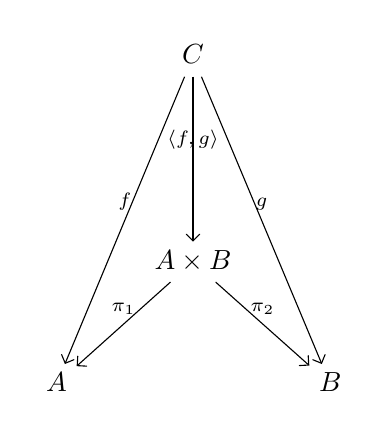
\begin{tikzpicture}[>=angle 90]
\matrix(a)[matrix of math nodes,
row sep=3em, column sep=2.5em,
text height=1.5ex, text depth=0.25ex]
{
&C& \\
\\
&A \times B&\\
A&&B\\};
\path[->,font=\scriptsize](a-1-2) edge node[above]{$f$} (a-4-1);
\path[->,font=\scriptsize](a-1-2) edge node[above]{$g$} (a-4-3);
\path[->,font=\scriptsize](a-1-2) edge node[above]{$\langle f, g\rangle$} (a-3-2);
\path[->,font=\scriptsize](a-3-2) edge node[above]{$\pi_1$} (a-4-1);
\path[->,font=\scriptsize](a-3-2) edge node[above]{$\pi_2$} (a-4-3);
\end{tikzpicture}
\caption{Product}
\end{figure}

\begin{figure}
\begin{tikzpicture}[>=angle 90]
\matrix(a)[matrix of math nodes,
row sep=3em, column sep=2.5em,
text height=1.5ex, text depth=0.25ex]
{
A&&B \\
&F\ \Downarrow &\\
F A&&F B\\};
\path[->,font=\scriptsize](a-1-1) edge node[above]{$f$} (a-1-3);
\path[->,font=\scriptsize](a-1-1) edge node[left]{$F$} (a-3-1);
\path[->,font=\scriptsize](a-1-3) edge node[right]{$F$} (a-3-3);
\path[->,font=\scriptsize](a-3-1) edge node[above]{$F f$} (a-3-3);
\end{tikzpicture}
\caption{Functor}
\end{figure}

\begin{figure}
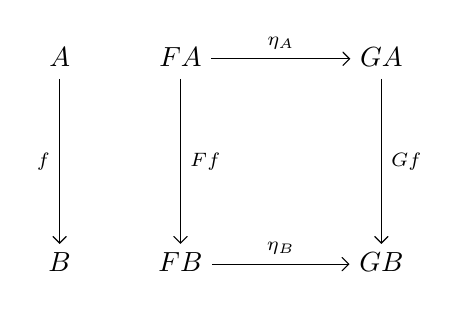
\begin{tikzpicture}[>=angle 90]
\matrix(a)[matrix of math nodes,
row sep=3em, column sep=2.5em,
text height=1.5ex, text depth=0.25ex]
{
A&F A &&G A \\
& &&\\
B&F B&&G B\\};
\path[->,font=\scriptsize](a-1-1) edge node[left]{$f$} (a-3-1);
\path[->,font=\scriptsize](a-1-2) edge node[above]{$\eta_A$} (a-1-4);
\path[->,font=\scriptsize](a-1-2) edge node[right]{$F f$} (a-3-2);
\path[->,font=\scriptsize](a-1-4) edge node[right]{$G f$} (a-3-4);
\path[->,font=\scriptsize](a-3-2) edge node[above]{$\eta_B$} (a-3-4);
\end{tikzpicture}
\caption{Natural Transformation}
\end{figure}

\begin{figure}
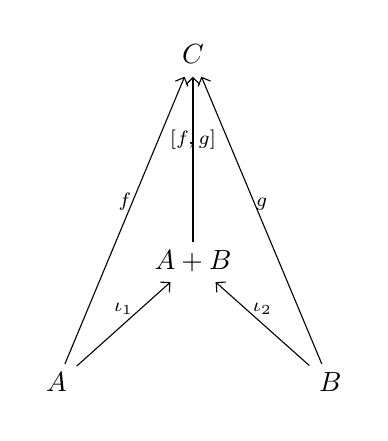
\begin{tikzpicture}[>=angle 90]
\matrix(a)[matrix of math nodes,
row sep=3em, column sep=2.5em,
text height=1.5ex, text depth=0.25ex]
{
&C& \\
\\
&A + B&\\
A&&B\\};
\path[<-,font=\scriptsize](a-1-2) edge node[above]{$f$} (a-4-1);
\path[<-,font=\scriptsize](a-1-2) edge node[above]{$g$} (a-4-3);
\path[<-,font=\scriptsize](a-1-2) edge node[above]{$[f,g]$} (a-3-2);
\path[<-,font=\scriptsize](a-3-2) edge node[above]{$\iota_1$} (a-4-1);
\path[<-,font=\scriptsize](a-3-2) edge node[above]{$\iota_2$} (a-4-3);
\end{tikzpicture}
\caption{Sum (co-product)}
\end{figure}

\begin{figure}
\begin{tikzpicture}[>=angle 90]
\matrix(a)[matrix of math nodes,
row sep=3em, column sep=2.5em,
text height=1.5ex, text depth=0.25ex]
{
C \times A&&B \\
\\
&B^A \times A&\\};
\path[->,font=\scriptsize]
(a-1-1) edge node[above]{$f$} (a-1-3)
        edge node[left]{$\lambda f \times \mathrm{id}$} (a-3-2)
(a-3-2) edge node[right]{$\mathrm{ap}$} (a-1-3);
\end{tikzpicture}
\caption{Exponential}
\end{figure}

\begin{figure}
\begin{tikzpicture}[>=angle 90]
\matrix(a)[matrix of math nodes,
row sep=3em, column sep=2.5em,
text height=1.5ex, text depth=0.25ex]
{
A & &B \\
&& \\
C & &D \\};
\path[->,font=\scriptsize]
(a-1-1) edge node[above]{$f$} (a-1-3)
(a-1-1) edge node[left]{$g$} (a-3-1)
(a-3-1) edge node[above]{$f'$} (a-3-3)
(a-1-3) edge node[right]{$g'$} (a-3-3);
\end{tikzpicture}
\caption{Pullback}
\end{figure}


\end{document}
